\section{PENDAHULUAN}
\subsection{Latar Belakang}
    Seiring berkembangnya teknologi autonomous vehicles, terdapat banyak keinginan untuk mengaplikasikan teknologi tersebut di berbagai bidang.
    Salah satu aplikasi teknologi ini di bidang komersil adalah Amazon Prime Air.
    Amazon Prime Air memanfaatkan Autonomous Aerial Vehicle(AAV) untuk melakukan pengantaran barang dari warehouse ke rumah kostumer secara autonomous.

    Salah satu tantangan terbesar dari penerbangan autonomous adalah kemampuan Sense and Avoid (SAA) dari AAV.
    Meskipun di udara terdapat ruang gerak yang luas, tetap terdapat resiko AAV akan menabrak objek di udara.
    Objek - objek tersebut dapat berupa helikopter, pesawat, burung, misil, dan lain - lain.
    Objek - objek ini juga sering disebut dengan Objek Airborne. 

    Salah satu sensor yang dapat digunakan untuk melakukan SAA adalah kamera.
    Kamera memiliki bobot yang cukup ringan, sehingga dapat dibawah oleh AAV.
    Selain itu, kamera juga memiliki harga yang relatif lebih murah dibandingkan sensor - sensor seperti LiDAR atau Radar.
 
    Dengan memilih kamera sebagai sensor, maka dibutuhkan suatu model computer vision untuk diaplikasikan pada kamera tersebut.
    Objek - objek airborne akan tampak sangat kecil pada kamera.
    Beberapa dataset kamera airborne yang memiliki resolusi 20482448 pixel, objeknya dapat berukuran 4 (0.00008\% luas resolusi) hingga 1000 pixel (0.01\% luas resolusi) sehingga terlihat sangat kecil \parencite{aot_docs}.
    Oleh karena itu, dibutuhkan suatu model yang dapat mendeteksi objek - objek yang sangat kecil agar bisa mendeteksi objek airborne.

    \begin{figure} [ht]
        \centering
        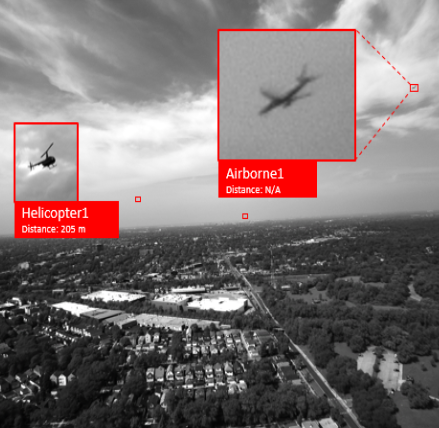
\includegraphics[scale=0.5]{pictures/dataset-example-labeled.png}
        \caption{Contoh Objek Airborne}
        \label{fig:airborne-object-example-1}
    \end{figure}

    YOLOv7 merupakan model state-of-the-art untuk melakukan pendeteksian objek secara real-time.
    YOLOv7 memiliki akurasi tertinggi dari semua model pendeteksi objek dengan kecepatan deteksi 30 FPS (yang terpublikasi) pada GPU Nvidia V100.
    Terdapat versi scaled dari YOLOv7 yang memiliki jumlah parameter yang lebih kecil dan dapat diaplikasikan pada device edge computing \parencite{yolov7}.
    Oleh karena itu, YOLOv7 ini cocok untuk digunakan pada AAV di mana dibutuhkan suatu pendeteksi objek yang real-time.

\subsection{Rumusan Masalah}
    YOLOv7 bukan merupakan model deteksi objek umum sehingga YOLOv7 tidak didesain untuk melakukan deteksi objek kecil seperti objek-objek \emph{airborne}.
    Oleh karena itu, dapat dibuat rumusan masalah seperti berikut:
    \begin{enumerate}
        \item Apa yang dapat dilakukan pada YOLOv7 untuk mengoptimisasi kemampuan deteksi objek airborne?
    \end{enumerate}

\subsection{Tujuan}
    Adapun tujuan dari tugas akhir ini adalah:
    \begin{enumerate}
        \item Untuk menemukan metode untuk mengoptimisasi kemampuan YOLOv7 mendeteksi objek airborne.
    \end{enumerate}

\subsection{Batasan Masalah}
    lorem ipsum dolor






